\documentclass[12pt]{article}
\usepackage{amsfonts,listings,float,url}
\usepackage[pdftex]{graphicx}
\usepackage[english]{babel}
\usepackage{natbib}
\usepackage{url}
\usepackage[utf8x]{inputenc}
\usepackage{soul}
\usepackage{amsmath}
\usepackage{graphicx}
\graphicspath{{Mis/}}
\usepackage{parskip}
\usepackage{enumerate}
\usepackage{fancyhdr}
\usepackage{longtable}
\usepackage{vmargin}
\usepackage{chngpage}
\usepackage{array}
\usepackage{ulem}
\usepackage[T1]{fontenc}
\usepackage{booktabs}
\usepackage{units}
\usepackage{array}
\usepackage{blindtext}
\usepackage{tabularx}
\usepackage{booktabs}
\usepackage[table,xcdraw]{xcolor}
\usepackage{listings}
\usepackage{multirow}
\usepackage{graphicx,wrapfig,lipsum}
\usepackage{caption, fancyhdr}
\definecolor{mygreen}{RGB}{28,172,0} % color values Red, Green, Blue
\definecolor{mylilas}{RGB}{170,55,241}
\allowdisplaybreaks[1]

\lstset{language=Matlab,%
	%basicstyle=\color{red},
	basicstyle=\tiny,
	breaklines=true,%
	morekeywords={matlab2tikz},
	keywordstyle=\color{blue},%
	morekeywords=[2]{1}, keywordstyle=[2]{\color{black}},
	identifierstyle=\color{black},%
	stringstyle=\color{mylilas},
	commentstyle=\color{mygreen},%
	showstringspaces=false,%without this there will be a symbol in the places where there is a space
	numbers=left,%
	numberstyle={\tiny \color{black}},% size of the numbers
	numbersep=9pt, % this defines how far the numbers are from the text
	emph=[1]{for,end,break},emphstyle=[1]\color{red}, %some words to emphasise
	%emph=[2]{word1,word2}, emphstyle=[2]{style},    
}

\newcommand{\ra}[1]{\renewcommand{\arraystretch}{#1}}
\newcolumntype{P}[1]{>{\centering\arraybackslash}p{#1}}
\setmarginsrb{3 cm}{2.5 cm}{3 cm}{2.5 cm}{1 cm}{1.5 cm}{1 cm}{1.5 cm}

\title{Consulting TAA}								% Title
\author{Drew Hollis \\ Xinyu Zhang \\ Qiang Heng}
% Author
\date{\today}											% Date

\makeatletter
\let\thetitle\@title
\let\theauthor\@author
\let\thedate\@date
\makeatother

\pagestyle{fancy}
\fancyhf{}
\rhead{\theauthor}
\lhead{\thetitle}
\cfoot{\thepage}
\lstset{language=R,
    basicstyle=\small\ttfamily,
    stringstyle=\color{DarkGreen},
    otherkeywords={0,1,2,3,4,5,6,7,8,9},
    morekeywords={TRUE,FALSE},
    deletekeywords={data,frame,length,as,character},
    keywordstyle=\color{blue},
    commentstyle=\color{DarkGreen},
}

\begin{document}
	
	%%%%%%%%%%%%%%%%%%%%%%%%%%%%%%%%%%%%%%%%%%%%%%%%%%%%%%%%%%%%%%%%%%%%%%%%%%%%%%%%%%%%%%%%%
	
	\begin{titlepage}
		\centering
		\vspace*{0.5 cm}
		
\includegraphics[scale = 0.2]{ncsu411.jpg}\\[1.0 cm]	% University Logo

		\textsc{\large ST841 Statistical Practice I}\\[0.5 cm]				% Course Name
		\rule{\linewidth}{0.2 mm} \\[0.4 cm]
		{ \huge \bfseries \thetitle}\\
		\rule{\linewidth}{0.2 mm} \\[1.5 cm]
		
		\textsc{	\begin{minipage}{0.4\textwidth}
				\begin{flushleft} \large
					\emph{Author:}\\
					\theauthor
				\end{flushleft}
			\end{minipage}~
			\begin{minipage}{0.4\textwidth}
				\begin{flushright} \large
					\emph{Contact Email:} \\
					anhollis@ncsu.edu \\
					xzhang97@ncsu.edu \\
					qheng@ncsu.edu
				\end{flushright}
			\end{minipage}\\[2 cm]
		}	
		{\large \thedate}\\[2 cm]
		
		\vfill
    \newpage		
	\tableofcontents
	\pagebreak
	\end{titlepage}
	
	%%%%%%%%%%%%%%%%%%%%%%%%%%%%%%%%%%%%%%%%%%%%%%%%%%%%%%%%%%%%%%%%%%%%%%%%%%%%%%%%%%%%%%%%%
	
	
	





\section{Introduction}


Businesses must take advantage of the latest technologies to stay relevant and competitive. Many new technologies and tools can automate mundane business administration tasks. Automating administrative tasks leads to greater efficiency and fewer errors and free up employees to focus on tasks that add more value to the company. All of these principles hold for a company's tax and accounting department as well. \\

The advent of robotic process automation (RPA), the automation of business processes using artificial intelligence and software, has had a particularly significant impact on the accounting profession. \cite{mezzio2019robotic} The extent to which companies and accounting departments have adopted and integrated automated tax tools into their workplace vary. Our client's study aims to determine what factors seem to have the most significant impact on the initiation, adoption, and routinization of tax analytics and automation (TAA) tools in larger companies. \\

Initiation, adoption, and routinization are explained in \cite{cooper1990information}.  Initiation refers to an initial evaluation of the suitability of technology by the company, adoption refers to the point at which a company recognizes technology as valuable for its interests and begins to integrate that technology into its business practices, and routinization refers to the full-scale deployment of that technology. \\

In determining what factors most impact the initiation, adoption, and routinization of a technology by a company, our client employed the technology-organization-environment (TOE) framework that first proposed in \cite{tornatzky1990process} and later used by \cite{zhu2006process} to study the diffusion of e-business technology in companies.\\

The TOE framework indicates that technology diffusion is influenced by the technological sophistication and preparedness of a company, the organizational and managerial attributes of a company, and the regulatory and competitive context or environment of a company. \\


%\hl{Do we wanna have these hypotheses? Since our %client's need might have changes and our reports do %not mentioned that so much, I prefer to hide those %hypothesis?}

Our client is interested in determining which of these factors are related to the three response variables initiation, adoption, and routinization. Our client has already done some preliminary analysis exploring the relationship of the above explanatory variables to routinization \cite{chen2020technology}. \\
%Our client is interested in testing five hypotheses %regarding TAA tools using the TOE framework:

%\begin{enumerate}
%\item Technology readiness is positively related to %TAA initiation/adoption/routinization.
%\item Technology integration is positively related to %TAA initiation/adoption/routinization.
%\item Managerial obstacles are negatively related to %TAA initiation/adoption/routinization.
%\item Competition intensity is positively related to %TAA initiation/adoption/routinization.
%\item A supportive regulatory environment is %positively related to TAA %initiation/adoption/routinization.
%\end{enumerate}


\subsection{Data}

To answer these questions, our client sent surveys to a chief tax officer at each of the Fortune 1000 companies asking about the initiation, adoption and routinization of TAA within that company's tax department and the level of technological readiness, technological integration, managerial obstacles, competition intensity, and regulatory support for TAA for the company. Of the 1000 companies that received surveys, 68 responded.\\

Several of the variables like initiation, routinization, managerial obstacles, technology integration, competition intensity, and regulatory environment were measured using a number of 5-point Likert scale survey items. For instance to measure initiation, respondents were asked to use a Likert scale on 7 survey items to rate the significance that each of 7 potential TAA benefits had in their initial decision to pursue TAA tools. \\

Other variables like technological readiness where measured by asking a series of questions relating to the kinds of technology used at the company and the number of tax employees at the company who specialize in the use of TAA tools. \\




\subsection{Survey Details and Preliminary Data Transformation}

The data were collected using a survey with 28 questions. Each survey question is listed in the table in Figure \ref{fig:dat} with a description of its format and the model variable it relates to.\\

Q6 asks the respondent to check all the levels (emerging, intermediate, and advanced) of TAA tools their company adopted and Q22 asks the respondent to check all specific TAA tools their company employs. Thus the responses to these questions are multiple checks corresponding to the technologies a company has employed. In order to turn these responses into a single numerical measure, we worked with the client to construct numerical weights corresponding to each check box. We then computed a weighted average across the check boxes for each observation to obtain a single numerical value summarizing the strength of each response for Q6 and Q22. \\

To obtain univariate measures for each of the Likert item questions, we performed nonlinear principal components analysis to a one-dimensional summary of each of the Likert scale questions. This procedure is described in detail in section 2.1.
\section{Methodology}

% \hl{Main description of the combination of the methodologies  -- XINYU} DONE!

In this section, we provide more theoretical backgrounds of the methodologies that we adopt in this consulting project for the convenience of the client's future replication and publication. Aside from theoretical supports for the client's future references in this report, we would also provide a separate runnable RMarkdown file for technical supports. This section has been divide into four parts. Section \ref{sec:likert} introduces how to combine the Multiple Likert Items into one score for the analysis using the non-linear Principal Component Analysis (PCA). Section \ref{sec:misimpute} describes the methodology for imputing the missing values using Amelia. Section \ref{sec:mlr} states the main framework of the multivariate regression analysis, which was also adopted by the client before. Besides, Section \ref{sec:tree} introduces the background of the regression tree methods, which were adopted to give more insights into the visualized tree.


\subsection{Creating Composite Scores from Multiple Likert Items} \label{sec:likert}

One challenge presented by the TAA dataset is that several response variables of interest like TAA evaluation and routinization and several explanatory variables of interest like technology integration and managerial obstacles are measured using multiple Likert scale items. \\

When several survey items are used to measure a single underlying variable, it is often desirable to have some way of combining the information from the several survey items into a single composite score representing the variable of interest. A common approach for deriving such composite scores is to obtain the principal components of the several survey items and use these principal components, especially the first principal component as the composite score \cite{henderson1990use}\cite{motallebzadeh2007neurocognitive}.\\

Our difficulty is that we are dealing with Likert items for which principal components analysis is not really well-defined. One solution to this problem is nonlinear principal components analysis with optimal scaling as described in \cite{linting2007nonlinear} and \cite{de2011multivariate}. This approach proceeds by finding an optimal transformation of the Likert data into a continuous representation and then performing standard PCA on this transformed representation. \\

Similar to standard principal components analysis, the nonlinear principal components analysis problem can be represented as a loss minimization problem. We minimize the loss function using a technique called alternating least squares. \\

Let $\textbf{X}_{n\times p}$ be a matrix of $n$ observations of $p$ Likert scale items. We assume that $x_{ij}$, the $i$-th observation of the $j$-th item is 1 for the lowest rank item on the Likert scale, 2 if it is the second lowest rank item on the Likert scale, and so on. This represents the raw Likert scale data we would like to condense into a composite score. Let $\textbf{Q}_{n \times p}$ represent the transformed version of $\textbf{X}$ under optimal scaling. Let $\textbf{H}_{n \times q}$ be the matrix of component scores where $q \leq p$. In our application, since we want a single composite score, we have $q=1$. Finally, let $\textbf{A}_{q \times p}$ be the matrix of component loadings. $\textbf{H}\textbf{A}$ can be interpreted as a rank $q$ approximation to $\textbf{X}$. We wish to find the optimal approximation, so we minimize the loss function:

\begin{equation}
L(\textbf{Q},\textbf{H},\textbf{A})=n^{-1} \sum_{j=1}^p (\textbf{q}_j-\textbf{H}\textbf{a}_j)^T(\textbf{q}_j-\textbf{H}\textbf{a}_j)
\end{equation}

where $\textbf{q}_j$ and $\textbf{a}_j$ are the $j$-th columns of $\textbf{Q}$ and $\textbf{A}$ respectively. Alternating least squares works by iteratively minimizing the loss function with respect to one of $\textbf{Q}$, $\textbf{H}$, or $\textbf{A}$ while holding the others constant until some convergence criterion is met. Thus, the optimal scaling problem (finding $\textbf{Q}$) is solved simultaneously with the principal components problem. \\

All that remains is to speak briefly about the form of $\textbf{Q}$. In general for each of $j=1,..,p$, we have

\begin{equation}
q_{ij}=\sum_{k=1}^b \alpha_k\phi_k(x_{ij})
\end{equation}

where $q_{ij}$ is the $i$-th entry of $\textbf{q}_j$ and $\phi_k(\cdot)$ is a basis function representation of $x_{ij}$. After some preliminary experimentation, a second degree B-spline was determined to do the best job of capturing the structure in the Likert items. If $x_{ij}$ is a missing value, $\phi_k(\cdot)$ is set to $1/b$. This is one of three methods for handling missing values suggested in \cite{de2011multivariate}. It is called the averaging method. After experimentation, it was found that the other two methods produced imputations for the missing values that were too extreme relative to the non-missing values. The optimization of the loss function with respect to $\textbf{Q}$ involves finding for each $j=1,...p$, the set of $\alpha_1,...,\alpha_k$ that minimizes the loss function. 

\subsection{Missing Value Imputation} \label{sec:misimpute}
\paragraph{Survey data} As introduced before, there are 28 survey questions in total, and 23 of which are selected based on the references and the client's subject knowledge.  

\begin{figure} [!hb]
 \centering 
 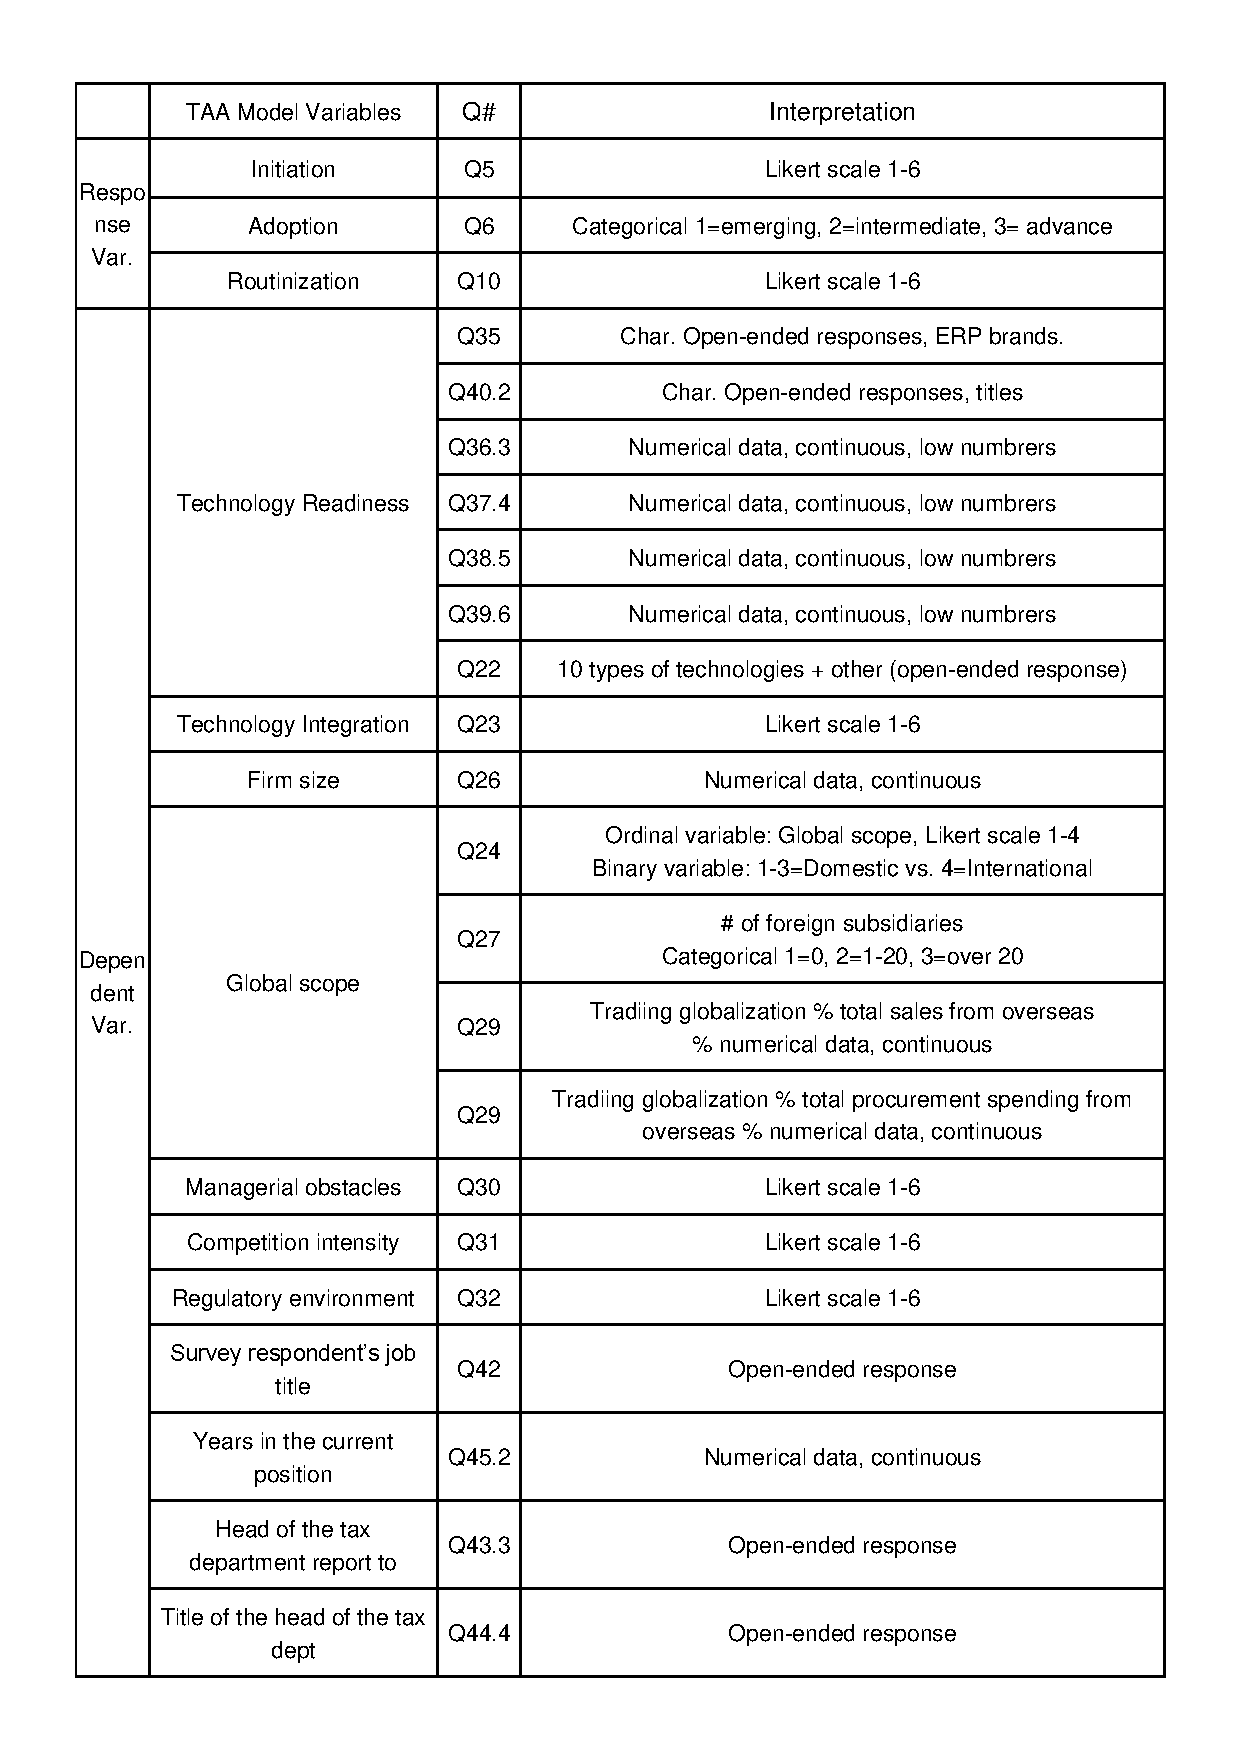
\includegraphics[width = .85\textwidth]{Mis/dat_Table.pdf}
 \caption{The mapping of useful survey questions to the variables for analysis }
 \label{fig:dat}
\end{figure}

\paragraph{Missing value for the original survey data:} 
We conducted an exploratory data analysis on this dataset with 68 observations and 56 original variables. We checked the proportion of missing values and have observed that there are fifteen variables that have a proportion of missing values larger than fifty percent; ten variables have the $10\%-50\%$ proportion of missing values; only the five categorical variables corresponding to Q5 have no missing value.  For Observations in row 1, 2, and 5, we could also notice they have almost all variables missing.


\begin{figure}[!h]
\centering
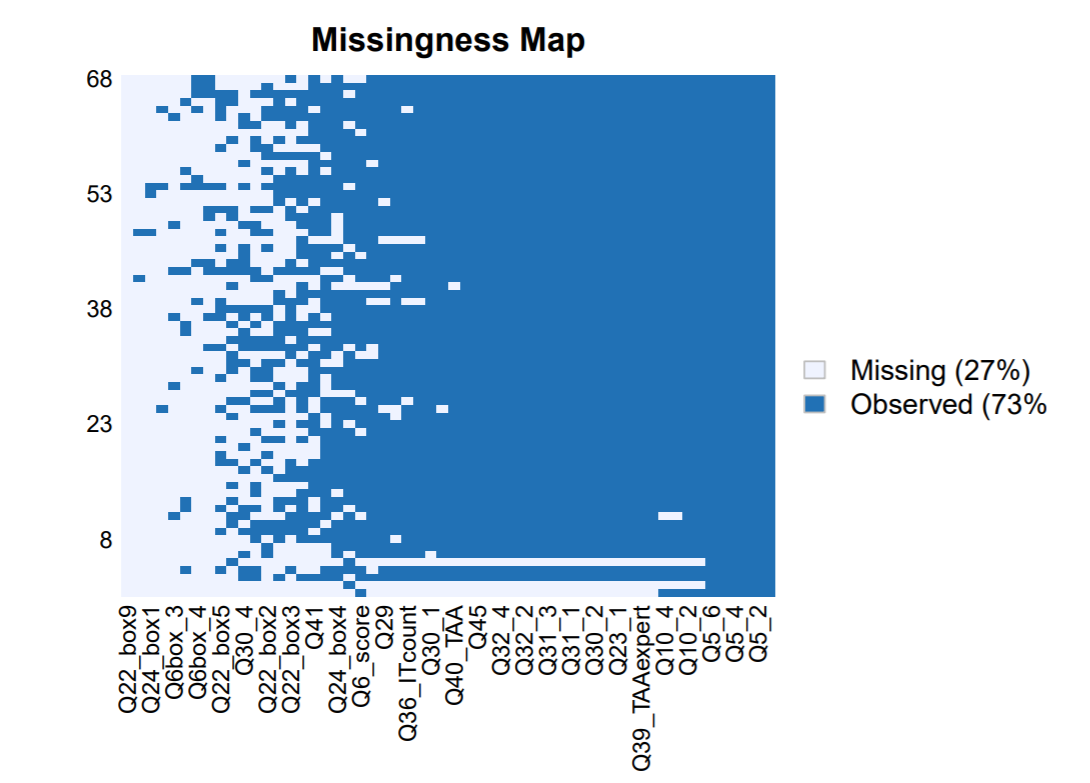
\includegraphics[width=.8\textwidth]{missmap.png}
\caption{The visualization of missingness in the data. The Y-axis is the id of the observation. The X-axis is the variables ordered with a decreasing proportion of missing values from left to right.}
\label{fig:missmap}
\end{figure}

Hence, after the discussion with the clients, we only keep 65 observations, and these 23 questions involve 56 variables mapping the ten variables, three response variables, and seven predictor variables as the table in Figure \ref{fig:dat} shows.

\begin{figure}[!h]
\centering
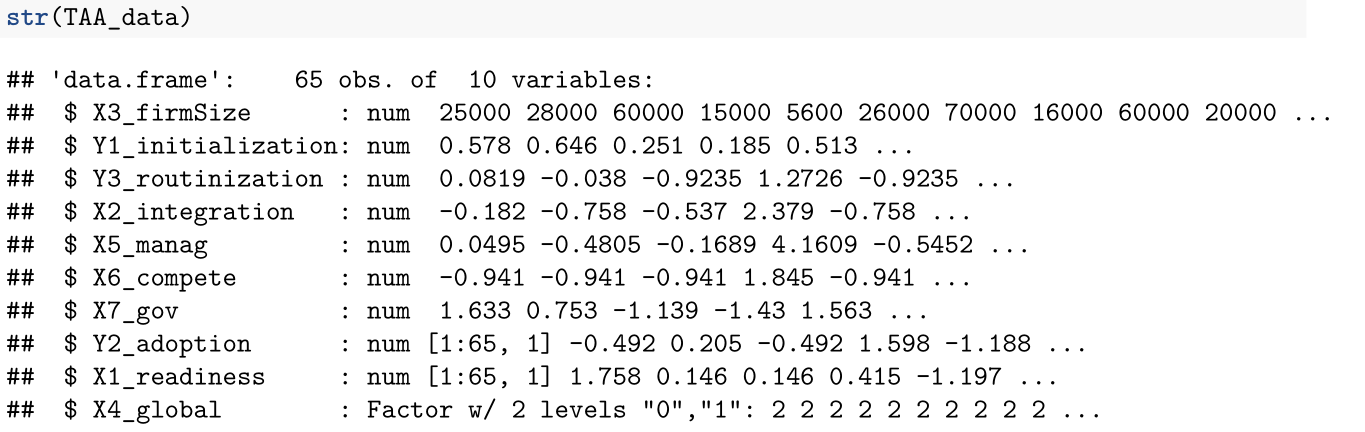
\includegraphics[width=.8\textwidth]{data.png}
\caption{Cleaned data for analysis}
\label{fig:missmap}
\end{figure}



\paragraph{AMELIA imputation method:} As for the missing value imputation, we adopt the method named AMELIA.  \cite{honaker2011amelia}
Here the method assumes the first assumption that the complete data $\mathcal{D}_{n \times k} = ( \mathcal{D}^{obs}, \mathcal{D}^{mis})$ follows the multivariate normal distribution, which is 

\begin{equation} \label{eq:norm}
    \mathcal{D} \sim N_k (\mu, \Sigma)
\end{equation}

and a second assumption that missing data are missing at random (MAR), which means the probability of missingness could be fully explained by observed data, defined as 
\begin{equation} \label{eq:mar}
    p(M \mid \mathcal{D}) = p(M \mid \mathcal{D}^{obs})
\end{equation}

where M is the missing matrix with $M_{ij} = I(\mathcal{D}_{ij} \in \mathcal{D}^{mis})$.

Hence, the normal assumption as well as the MAR assumption should be checked after the data are fully prepared and before the conduction of imputation.

Remembering the normality assumption Eq. \ref{eq:norm} and the missing at random assumption Eq. \ref{eq:mar}, we can obain the following likelihood for the observed data $\mathcal{D}^{\mathrm{obs}}$:

\begin{equation}
p\left(\mathcal{D}^{\mathrm{obs}}, M \mid \theta\right)=p\left(M \mid \mathcal{D}^{\mathrm{obs}}\right) p\left(\mathcal{D}^{\mathrm{obs}} \mid \theta\right)
\end{equation}


where $\theta=(\mu, \Sigma)$ is the parameter of interest. Thus the likelihood of $\theta$ based on observed data can be expressed as:

\begin{equation}
L\left(\theta \mid \mathcal{D}^{\mathrm{obs}}\right) \propto p\left(\mathcal{D}^{\mathrm{obs}} \mid \theta\right)
=\int p(\mathcal{D} \mid \theta) d \mathcal{D}^{\mathrm{mis}}
\end{equation}


and with a uniform prior of $\theta$, the posterior could be

\begin{equation}
    p\left(\theta  \mid  \mathcal{D}^{\mathrm{obs}} \right)
\propto \int p(\mathcal{D} \mid \theta) d \mathcal{D}^{\mathrm{mis}}
\end{equation}


Since the $\mathcal{D}^{\mathrm{mis}}$ is missing, Expectation-Maximization (EM) algorithm combined with a bootstrap approach is applied here to obtain the estimated modes of the posterior with its variance estimation. By assuming a start point of $\theta_0$, we define the Q function as

\begin{equation}
  Q(\theta \mid \theta^{v}) = E_{\theta^{v}}(ln(p\left(  \mathcal{D} \mid \theta \right)) \mid  \mathcal{D}^{\mathrm{obs}})
\end{equation}


where $p\left(  \mathcal{D} \mid \theta \right)$ is the complete data likelihood. The updates of $\theta^{v+1}$ given $\theta^{v}$ as 

\begin{equation}
 \theta^{v+1} = \arg \max_{\theta} Q(\theta \mid \theta^{v})
\end{equation}

Thus, we have the estimations of $\theta$ and can make imputation of the missing data based on the observed data as well as the estimated parameters for the complete data likelihood.

Besides, $m$ simultaneous imputations can be combined together to produce a more stable average imputaion:

\begin{equation}
\bar{T}=\frac{1}{m} \sum_{j=1}^{m} T_{j}
\end{equation}

where $j$  represents the $j^{th}$ datasets, and the $\bar{T}$ has the following standard error:


\begin{equation}
S E(T)= \sqrt{ \frac{1}{m} \sum_{j=1}^{m} S E\left(T_{j}\right)^{2}+S_{T}^{2}(1+1 / m) }
\end{equation}


where, $S_{T}^{2}=\Sigma_{j=1}^{m}\left(T_{j}-\bar{T}\right)^{2} /(m-1)$ is the sample variance across the m estimations, and $S E\left(T_{j}\right)^{2}$ is the estimated variance of $T_j$ based on the $j^{th}$ dataset.


Besides, it's also common that to treat the missing value of a categorical variable as a new variable; for the questions related to Likert scales where there's always a level that indicating the customer doesn't know the answer, we can directly change the missing value into that case; some times a mean imputation would also be appropriate if sufficient subject knowledge is grounded. Thus, the missing value imputation of this project can be quite customized to the specific variable with more subject knowledge. However, cleaner data should be get in the first step.


\subsection{Multi-response (Multivariate) Linear Regression} \label{sec:mlr}
% \hl{We decided to delete three observations with too many covariates missing.}
A common technique for handling multiple responses is multi-response (multivariate) linear regression. Suppose we have $m$ responses with $p$ features and $n$ observations, multi-response linear regression can be written in matrix form
\begin{equation}
Y=XB+E
\end{equation}
where $Y\in\mathbb{R}^{n\times m}$ are the dependent variables, $X\in\mathbb{R}^{n\times p}$ are the independent variables, $B\in\mathbb{R}^{p\times m}$ are the coefficients and $E\in\mathbb{R}^{n\times m}$ are the errors. To account for the possible correlation of different columns of $Y$, we assume that each row $E_{i.}$ of $E$ has a covariance matrix $\Sigma\in \mathbb{R}^{m\times m}$. If put in vectorized form,
\begin{equation}
\operatorname{vec}(Y)|X\sim \mathcal{N}([B'\otimes I_n]\operatorname{vec}(X),\Sigma \otimes I_n)
\end{equation}
It can be shown that the maximum likelihood estimate of $B$ is invariant to $\Sigma$, which can be computed using ordinary least square
\begin{equation}
\hat{B}=(X'X)^{-1}X'Y
\end{equation}
Then an unbiased estimate of error covariance matrix $\Sigma$ is given by
\begin{equation}
\hat{\Sigma}=\frac{Y'(I_n-X(X'X)^{-1}X')Y}{n-p}
\end{equation}
while the MLE for $\Sigma$ is given by
\begin{equation}
\tilde{\Sigma}=\frac{Y'(I_n-X(X'X)^{-1}X')Y}{n}
\end{equation}
The least square estimate $\hat{B}$ has the following distribution 
\begin{equation}
\operatorname{vec}(\hat{B})\sim \mathcal{N} (\operatorname{vec}(B),\Sigma\otimes(X'X)^{-1})
\end{equation}
Thus if we want to test $B_{jk}=0$ against $B_{jk}\ne0$, it can be seen that
\begin{equation}
\frac{\hat{B}_{jk}}{\hat{\Sigma}_{kk}(X'X)^{-1}_{jj}}\sim t_{n-p}
\end{equation}
which will provide a p value for each regression coefficient $B_{jk}$. It is worth pointing out that mathematically, statistical inference for a single entry $B_{jk}$ in the coefficient matrix $B$ is the same for single-response linear regression and multi-response linear regression. However, compared with separate single-response linear regression models, multi-response linear regression takes possible correlation of response columns into consideration, which will enable inference for blocks of $B$. For example, we might be interested in testing whether several independent variables have a joint significant impact on all the response variables, i.e. we want to test whether a reduced model with $q<p$ covariates is sufficient. The hypotheses can be formulated as
\begin{equation}\label{hypotheses}
    H_0: B_2=0 \text{ versus } H_1: B_2\ne 0
\end{equation}
where $B_2\in \mathbb{R}^{(p-q)\times m}$ is a part of the partitioned $B=\begin{pmatrix}B_1 \\ B_2\end{pmatrix}$. Then the likelihood ratio statistic becomes
\begin{equation}
\Lambda=\frac{\underset{B_1,\Sigma}\sup\; L(B_1,\Sigma)}{\underset{B,\Sigma}\sup\; L(B,\Sigma)}=(\frac{|\tilde{\Sigma}|}{|\tilde{\Sigma}_1|})^{n/2}
\end{equation}
where $\tilde{\Sigma}_1$ and $\tilde{\Sigma}$ are respectively constrained and unconstrained MLEs for $\Sigma$. For large enough $n$, the modified likelihood ratio test statistic has an approximate chisquare distribution
\begin{equation}
-\nu \log(\Lambda) \sim \chi^2_{m(p-q)}
\end{equation}
where $\nu=n-p-\frac{1}{2}(m-p+q+2)$. \\
If we use $E$ to denote $n\tilde{\Sigma}$ and $H$ to denote $n(\tilde{\Sigma}_1-\tilde{\Sigma})$, statistics from the Multivariate Analysis of Variance (MANOVA) literature \cite{warne2014primer} which rely on F-distribution approximations can be adopted for testing \eqref{hypotheses}. Let $\lambda_1\ge\lambda_2\ge\dots\ge\lambda_p$ denote the eigenvalues of matrix $HE^{-1}$,
\begin{itemize}
    \item $\text{Wilk's lambda}=\sum_{i=1}^p \frac{1}{1+\lambda_i}=\frac{|E|}{|E+H|}$ 
    \item $\text{Pillai's trace}=\sum_{i=1}^p \frac{\lambda_i}{1+\lambda_i}=\operatorname{tr}(H(H+E)^{-1})$
    \item $\text{Hotelling-Lawley's trace}=\sum_{i=1}^p \lambda_i=\operatorname{tr}(HE^{-1})$
    \item $\text{Roy's largest root}=\max(\lambda_i)$
\end{itemize}
After the above test statistics are calculated, they are transformed into an F-statistic which will have an approximate or exact F-distribution under the null hypothesis. In some cases, the four tests are identical, which means they will lead to the same F-statistics and probabilities. When they do differ, Pillai's trace is often used because of its power and robustness \cite{carey1998multivariate}. We will take advantage of implementations of these tests in \lstinline{anova} function of \lstinline{stats} package in R \cite{team2013r} for our statistical computation.

\subsection{Regression Trees}\label{sec:tree}
Due to the outliers, missing values, and lack of normality in the data, we believed it was worthwhile to also employ regression methodology that was robust to these problems. \\

Regression trees \cite{hastie2015statistical} are a modelling framework that make fewer assumptions than linear regression models, automatically handle missing values without using imputation or ignoring data, are robust to outliers, and do not require the data to be normally distributed. \\

A regression tree is constructed by assigning each observation to a bin based on the values of the independent variables associated with that observation. The tree model predicts the response of a particular observation to be the mean of the responses in that observation's assigned bin. \\

The bins, or leaf nodes, are found by recursively splitting the set of observations on values of the independent variables so that at each split the prediction error in the resulting bins is minimized.\\

We illustrate a regression tree in figure \ref{fig:reg_tree}. The tree begins by splitting on the independent variable A. Observations with $A>2$ go to the left, observations with $A \leq 2$ go to the right. On the left the next optimal split is performed on variable B. The boxes at the bottom of the tree represent the leaf nodes. $P$ is the number of observations in that box and mean is the mean of the responses for those observations which is used as the prediction value.

\begin{figure}[H]
\centering
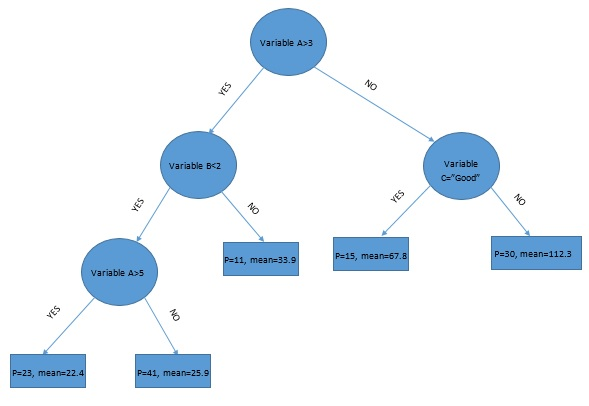
\includegraphics[width=0.8\textwidth]{decision_tree_illustrated.jpg}
\caption{Regression Tree Illustrated}
\label{fig:reg_tree}
\end{figure}

The splitting variables and the values for those variables that are used to define the split are chosen to optimize

$$
\sum_{i \in B} \sum_{j=1}^{p_i} (y_{ij}-\bar{y}_i)^2
$$

where $B$ is the set of boxes, $p_i$ is the number of observations in box $i$ and $\bar{y}_i$ is the mean of the responses for the observations in box $i$.


\section{Results}
 In this section we presents results of likert scale data transformation, mulvariate linear regression and regression trees. We first present graphs of likert scale item loadings to visualize how each item contributes to its composite score. Then we look at multivariate regression results to get an idea of how independent variables influence dependent variables. Taking possible correlation between response variables into consideration, MANOVA likelihood ratio tests are also conducted to see which independent variables have a significant impact on at least one of the response variables. Finally we create a regression tree for each response variable as a nonparametric alternative in our methodologies. The results of the regression trees are consistent with our findings in multivariate linear regression.

\subsection{Transformation of Likert Scale Data}
After using non-linear PCA to construct scores for the Likert data, it is useful to look at the loadings for each of the first principal component scores being used as a one-dimensional approximation. The loadings quantify the strength and direction of the relationship between each of the original Likert scale items and the first principal component. These loadings are depicted for each of the 6 Likert scale sets in Figure \ref{fig:loadings}.\\

\begin{figure}[H]
\centering
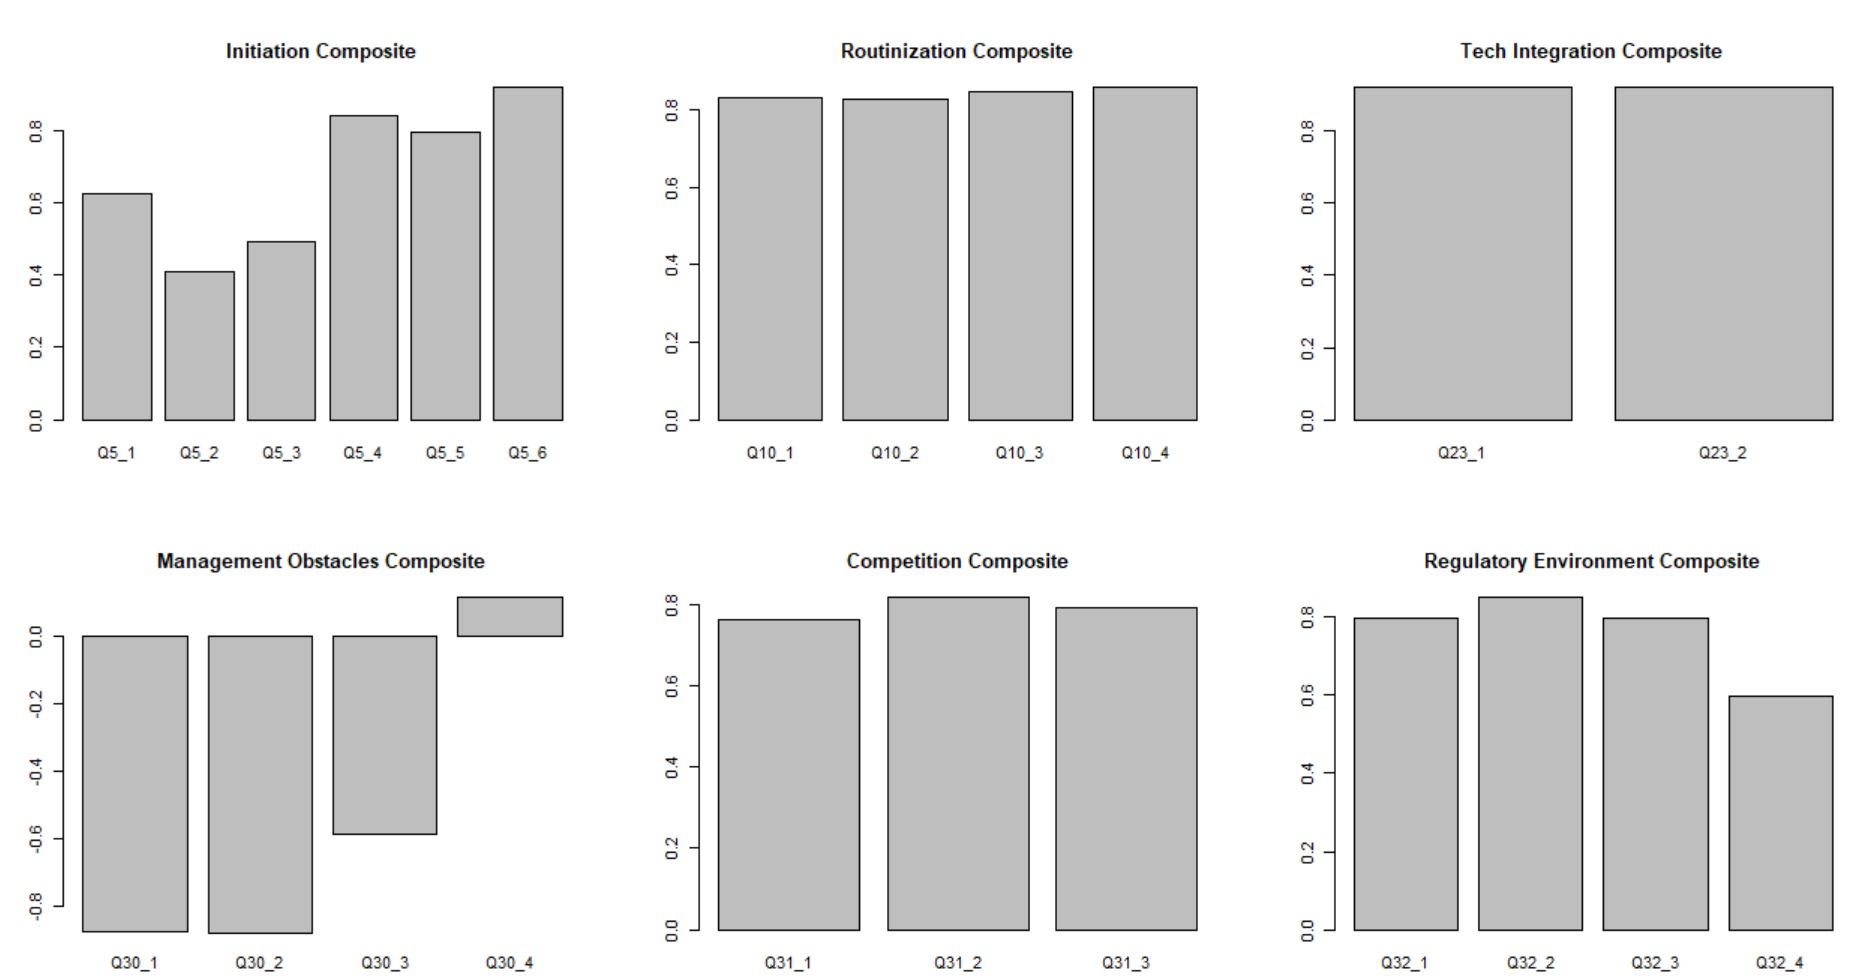
\includegraphics[width=0.8\textwidth]{loadings.jpg}
\caption{First Principal Component Loadings}
\label{fig:loadings}
\end{figure}

We can use the loadings plot in Figure \ref{fig:loadings} to help us interpret the meaning of the scores that we use to represent each of the 6 variables underlying the Likert scale items. For instance, from the first plot, we can see that the score representing the consideration a firm initially gives to considering different TAA technologies is most influenced by a company's responses to the fourth, fifth, and sixth Likert items. The first, second, and third questions relate to using TAA to reduce costs, expand in-house tax services, and improve the coordination of the tax department with other departments. The last three items relate to improving the reporting, analysis, and productivity of the tax department. We can see that the last three items relate more to the primary output of the tax department and the first three relate to how the operations of the tax department within the company. This provides insight into what the unified score is really measuring. It may be a measure of the role accounting department output played in a company's initial considerations for adopting TAA. \\

Another interesting variable is the management obstacles variable. For this variable, the firms rarely answered the fourth Likert question. Thus, this question was mostly missing values. This explains its almost negligible impact on the first principal component score. It is also interesting to note that the other questions have a negative relationship with the first principal component. Thus, for the managerial obstacles variable, we would interpret a lower score as indicating more significant managerial obstacles. 


\subsection{Multi-response (Multivariate) Linear Regression Results}
Recall that out response variables are TAA technology initiation, adoption and routinization, our independent variables are technology readiness, technology integration, firm size, global scope, management obstacles, competition intensity and regulatory environment. The explanatory variables are standardized to make the coefficients comparable and exclude intercepts from our model. The following table summarizes the coefficient estimates and their corresponding significance level. 
\begin{table}[H]
\centering
\begin{tabular}{|c|c|c|c|}
\hline
                       & Initiation & Adoption  & Routinization \\ \hline
Technology Readiness   & -0.11      & $0.50^{***}$ & 0.12          \\ \hline
Technology Integration & -0.06      & -0.05     & $0.33^{**}$      \\ \hline
Firm Size              & 0.06       & $0.26^*$    & -0.03         \\ \hline
Global Scope           & $0.37^{**}$  & -0.18     & 0.07          \\ \hline
Management obstacles   & -0.11      & 0.19      & 0.15          \\ \hline
Competition Intensity  & 0.07       & -0.01     & 0.14          \\ \hline
Regulatory Environment & 0.06       & 0.05      & 0.15          \\ \hline
\end{tabular}
\caption{Coefficients and their siginifice levels. *** means $p<0.001$, ** means $p<0.01$ and $*$ means $p<0.05$.}
\end{table}
Notice that significant coefficients are rare.  Now, let's utilize previously mentioned F-tests from MANOVA theory to decide whether a specific explanatory variable has a significant impact on all of the response variables. In other words, we can provide a single p value for each independent variable. The following table summarizes test statistics, the transformed F-statistics and their corresponding p values. Notice that in our case, the four tests, namely Wilk's lambda, Pillai's trace, Hotelling-Lawley's trace and Roy's largest root are equivalent and they produce the same F-statistics and p values, so we only report one F-statistic and p value for each independent variable. Also, Hotelling-Lawley's trace and Roy's largest root turn out to have identical test statistics, so we report them in one column.
\begin{table}[H]
\begin{tabular}{|c|c|c|c|c|c|c|}
\hline
                       & Wilk & Pillai & Hotelling/Roy   & F-statistic & p-value        \\ \hline
Technology Readiness   & 0.73 & 0.28   & 0.38              & 7.47        & $0.0003^{***}$ \\ \hline
Technology Integration & 0.86 & 0.14   & 0.16              & 3.10        & $0.03^{*}$     \\ \hline
Firm Size              & 0.90 & 0.10   & 0.11              & 2.07        & 0.11           \\ \hline
Global Scope           & 0.86 & 0.14   & 0.17              & 3.29        & $0.03^*$       \\ \hline
Management Obstacles   & 0.91 & 0.09   & 0.10              & 1.96        & 0.13           \\ \hline
Competition Intensity  & 0.98 & 0.02   & 0.03              & 0.50        & 0.68           \\ \hline
Regulatory Environment & 0.97 & 0.03   & 0.03              & 0.54        & 0.65           \\ \hline
\end{tabular}
\caption{MAONVA test statistics and their p values. *** means $p<0.001$, ** means $p<0.01$ and $*$ means $p<0.05$.}
\label{tab:my-table}
\end{table}
From the table we can see that technology readiness, integration and global scope are statistically significant. Firm size is significant for adoption but not significant overall. We can also see that management obstacles, competition intensity and regulatory environment don't seem to have significant impact on the response variables.

\subsection{Regression Trees}
We fit a separate regression tree for each of the three response variables. The resulting trees are plotted in the below figures. 

\begin{figure}[H]
\centering
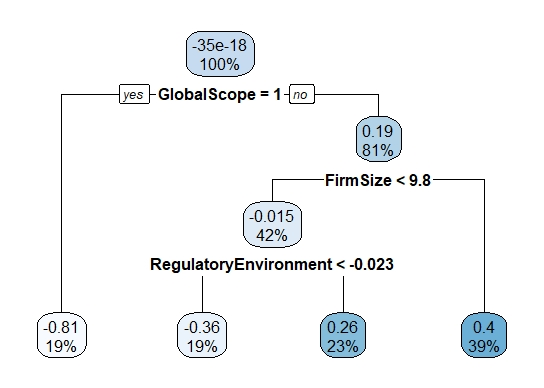
\includegraphics[width=0.8\textwidth]{init_tree.jpeg}
\caption{Initiation Tree}
\label{fig:init_tree}
\end{figure}

\begin{figure}[H]
\centering
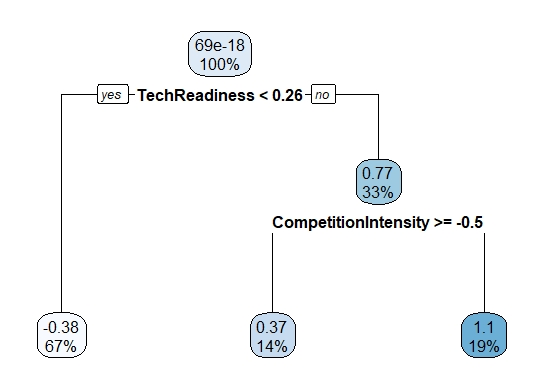
\includegraphics[width=0.8\textwidth]{adopt_tree.jpeg}
\caption{Adoption Tree}
\label{fig:adopt_tree}
\end{figure}

\begin{figure}[H]
\centering
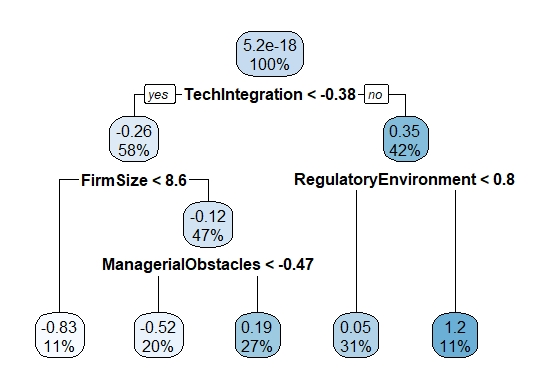
\includegraphics[width=0.8\textwidth]{rout_tree.jpeg}
\caption{Routinization Tree}
\label{fig:rout_tree}
\end{figure}

The first number in each box is the mean response for that partition of the tree and the percentage is the percentage of observations assigned to that partition of the tree. Thus, for the initiation tree, $19\%$ of the observations were purely domestic and these domestic firms had a mean initiation score of -0.81. $42\%$ had a foreign presence a log firm size less than 9.8 and a corresponding mean initiation score of -0.015, while $39\%$ of firms had a foreign presence and log firm size of more than 9.8 and a corresponding mean initiation score of 0.4.    

The first splitting variable is often interpreted as the most important or influential variable in the model. The results agree with the linear regression results in that for initiation the global extent of the firm as measured in global scope seems to be most associated with higher initial consideration of TAA, for adoption, technological readiness seems to be most closely associated with adopting more advanced TAA tools, and for routinization, technological integration seems to be most closely associated with better TAA routinization. \\


The variables lower down in the tree, however, may not be important, and may show up as being valuable only for partitioning this particular data set. The lower-level variables may not be generally important. 

\section{Discussion}

In this project, we provide multi-aspect statistical supports to help the client gain better understandings of the diffusion of tax automation techniques and develop better methodology in presenting the analysis in the research paper. We transformed the Likert scale using non-linear PCA; imputed the missing values using AMELIA through EM algorithm; analyzed the results using both multivariate linear regression for significant levels and regression tree analysis for interpretable visualizations. \\

It is important to note that the data set is small, there are outliers, and much of the data is missing. The linear regression results should be interpreted with caution due to the outliers, the small data set size, and the fact that the data don't appear to be normal. \\

While regression trees are robust many of these weaknesses, single-fit regression trees tend to over-fit the data. This issue may be exacerbated by the small sample size. The splitting variables lower down in the trees may not be generally important, and may show up as being valuable only for partitioning this particular data set.\\

Both our analyses have consistently identified a number of important variables for each of the stages of technology diffusion, and these findings may serve as a good basis for future studies. Because of some of the issues with the dataset mentioned above, however, we encourage the reader to interpret the results with some caution. \\


Also, we would provide an RMarkdown file aside from this report to the client as a documentary of replicable results for future research.



\bibliography{references}
\bibliographystyle{plain}

\end{document}
